\documentclass[
%%%%% Styles and Sizes
%10pt,
%11pt,
%12pt,
fancyheadings, % headings with seplines and logo
%
%%%%% Printing, Color and Binding
%a4paper, 
%a5paper,
%twoside, % single sided printout
%oneside, % duplex printout (default)
%% binding correction is used to compensate for the paper lost during binding
%% of the document
%BCOR=0.7cm, % binding correction
%nobcorignoretitle, % do not ignore BCOR for title page
%% the following two options only concern the graphics included by the document
%% class
%grayscaletitle, % keep the title in grayscale
%grayscalebody, % keep the rest of the document in grayscale
%
%%%%% expert options: your mileage may vary
%baseclass=..., % special option to use a different document baseclass
]{stsreprt}

% Information for the Titlepage
\author{Robin Willenbrock}
\title{Static Detection of Data Races in Interrupt-Driven Software Using Reduced Inter-Procedural Control Flow Graphs}
\date{\today}
\subject{Bachelor Thesis}
\professor{Prof. Dr. Sibylle Schupp }
\advisor{Ulrike Engeln}

\usepackage[utf8]{inputenc}
\usepackage{listings}
\usepackage{amsmath}
\usepackage{xcolor}
% Font and Fontencoding Magic
% FAQ: 
% http://tex.stackexchange.com/questions/664/why-should-i-use-usepackaget1fontenc
% http://en.wikipedia.org/wiki/Computer_Modern
% http://tex.stackexchange.com/questions/1390/latin-modern-vs-cm-super
\usepackage[T1]{fontenc}
\usepackage{lmodern}
%\usepackage{fix-cm}
\lstset{
	language=Python,
	basicstyle=\ttfamily\footnotesize,
	keywordstyle=\color{blue},
	commentstyle=\color{green},
	stringstyle=\color{red},
	numbers=left,
	numberstyle=\tiny\color{gray},
	stepnumber=1,
	numbersep=5pt,
	frame=single,
	breaklines=true,
	showstringspaces=false,
	tabsize=4,
	captionpos=b
}
\usepackage{tikz}
\usetikzlibrary{shapes.geometric, arrows, positioning}
\usepackage{caption}
\usepackage{float}
\usepackage[linesnumbered,ruled,vlined]{algorithm2e}
\raggedbottom

\tikzstyle{startstop} = [rectangle, rounded corners, minimum width=3cm, minimum height=1cm,text centered, draw=black, fill=red!30]
\tikzstyle{process} = [rectangle, minimum width=3cm, minimum height=1cm, text centered, draw=black, fill=orange!30]
\tikzstyle{decision} = [diamond, minimum width=3cm, minimum height=1cm, text centered, draw=black, fill=green!30]
\tikzstyle{arrow} = [thick,->,>=stealth]
\tikzstyle{redarrow} = [thick,->,>=stealth,draw=red]

% Package for Abbreviations
\usepackage{acronym}
\usepackage{hyperref} 

\begin{document}
	\frontmatter
	\maketitle
	\tableofcontents
	\listoffigures{}
	
	% Abbreviations
	\chapter*{Abbreviations}
	\begin{acronym}
		\acro{ISR}{Interrupt Service Routine}
		\acro{CFG}{Control Flow Graph}
		\acro{ICFG}{Inter-Procedural Control Flow Graph}
		\acro{RICFG}{Reduced Inter-Procedural Control Flow Graph}
		\acro{GCC}{GNU Compiler Collection}
		\acro{DFS}{Depth-First Search}
		\acro{BB}{BasicBlock}
	\end{acronym}
	
	\mainmatter{
		\chapter{Introduction}
		
		\chapter{Background}
		In this chapter, I am going to provide a brief overview of all the necessary background information needed to understand static data races in interrupt-driven software using \acp{RICFG}. This information includes basics about interrupt-driven systems, shared resources, \acp{RICFG}, and data races as a whole.
		
		\section{Interrupt-Driven Systems}
		An interrupt-driven system is an architecture where the flow of execution is changed by unpredictable events in the system, also known as interrupts. Interrupts can be caused by hardware devices, software conditions, or external signals, forcing the processor to suspend the current task to execute an interrupt handler or Interrupt Service Routine (\ac{ISR}). Interrupt-driven systems are used in real-time operating systems, embedded systems, and generally in systems where timely responses are necessary \cite{wang2020}.
		
		\begin{figure}[H]
			\centering
			\begin{tikzpicture}[node distance=2cm, scale=0.8, transform shape]
				
				\node (start) [startstop] {Start};
				\node (init) [process, below of=start] {Initialize System};
				\node (exec) [process, below of=init] {Execute Function};
				\node (interrupt) [decision, below of=exec, yshift=-0.8cm] {Interrupt Occurs?};
				\node (isr) [process, below of=interrupt, yshift=-0.8cm] {Execute \ac{ISR}};
				\node (resume) [process, below of=isr] {Resume Function};
				\node (end) [startstop, below of=resume] {End};
				
				\draw [arrow] (start) -- (init);
				\draw [arrow] (init) -- (exec);
				\draw [arrow] (exec) -- (interrupt);
				\draw [arrow] (interrupt) -- node[anchor=east] {Yes} (isr);
				\draw [arrow] (isr) -- (resume);
				\draw [arrow] (resume) -- (end);
				\draw [arrow] (resume.east) -- ++(1.5,0) node[anchor=north]  |- (exec.east);
				
			\end{tikzpicture}
			\caption{Flowchart of the Interrupt-Driven System}
		\end{figure}
		
		In Figure 2.1, a basic execution flow of a simple interrupt-driven system is displayed. The system executes a function as long as no interrupt occurs. When an interrupt occurs, it switches to the \ac{ISR}, executes it, and then resumes the function executed before the interrupt happened.
		
		The management of interrupts to maintain the fast responsiveness of the system is the most challenging part of an interrupt-driven system. Interrupts occur in unpredictable ways, so you have to consider every possible execution flow. To ensure the execution of critical interrupts, interrupts are often prioritized, so higher-priority events can interrupt lower ones and be handled immediately. When handling an interrupt, the current state of the processor is saved, and the context is switched to the \ac{ISR} \cite{wang2020}.
		
		The unpredictability and asynchronous nature of interrupts present many challenges in designing and implementing an interrupt-driven system. One of the biggest challenges is the correct handling of high-priority interrupts without delaying them substantially, which requires a sophisticated scheduling and prioritization mechanism. The execution of the main program and \ac{ISR} needs to be handled properly to ensure data integrity. 
		
		\section{Shared Resources}
		Analyzing the management of shared resources is a large part of data race analysis, which is further explained later. The following is a short introduction to shared resources to better understand them in the context of data races.
		
		Shared resources, often referred to as shared memory or shared variables, are data that can be accessed simultaneously by multiple threads or processes. Proper management of these resources is crucial because improper handling can lead to issues like data races, deadlocks, and other synchronization problems. In interrupt-driven systems, shared resources often involve variables or data structures that are accessed by both the main program and \acp{ISR}. Proper management of shared resources is critical to ensuring data consistency and avoiding conflicts \cite{herlihy2008}.
		
		Proper management of shared resources involves the use of synchronization mechanisms to coordinate access and ensure data consistency. Mutexes, semaphores, and condition variables are common tools used to control access to shared resources. Mutexes provide mutual exclusion, ensuring that only one thread can access the resource at a time. Semaphores can limit the number of threads accessing the resource simultaneously. Condition variables allow threads to wait for certain conditions to be met before proceeding, facilitating complex synchronization scenarios \cite{herlihy2008}. In interrupt-driven software, the synchronization of shared resources often involves disabling and enabling interrupts \cite{chopra2019}.
		
		\section{Reduced Inter-Procedural Control Flow Graphs}
		\acp{CFG} are representations of all possible paths through a program or function during its execution. An \acp{ICFG} adds possible edges between multiple programs or functions to also show possible control flows between those. A \ac{RICFG} is an optimized version of the ICFG that simplifies the graph to only the necessary information needed for the analysis \cite{engler2003}.
		
		\begin{figure}[H]
			\centering
			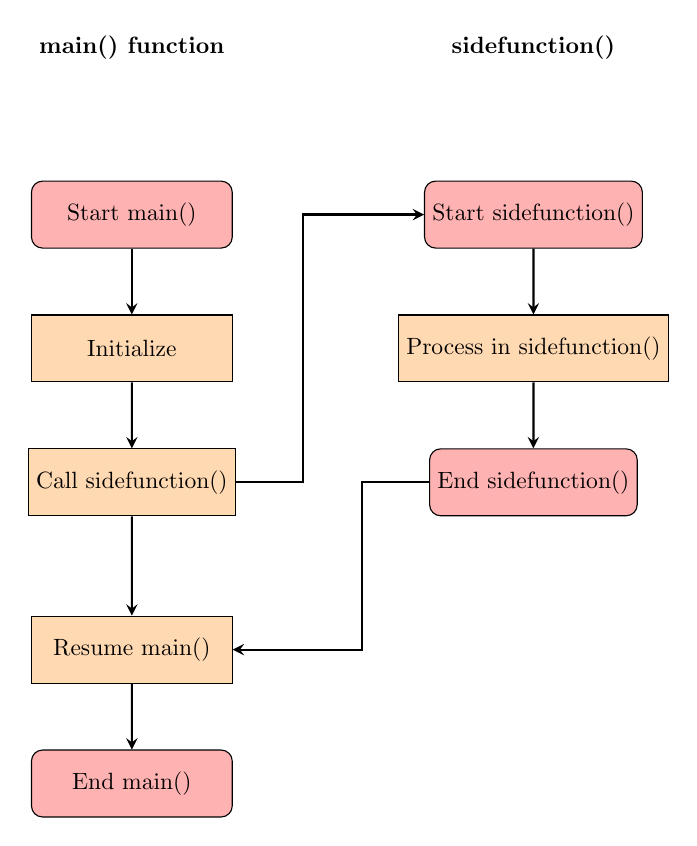
\begin{tikzpicture}[node distance=2cm, scale=0.85, transform shape]
				
				% Nodes for main function
				\node (start) [startstop] {Start main()};
				\node (init) [process, below of=start] {Initialize};
				\node (callsidefunction) [process, below of=init] {Call sidefunction()};
				\node (resume) [process, below of=callsidefunction, yshift=-0.5cm] {Resume main()};
				\node (end) [startstop, below of=resume] {End main()};
				
				% Nodes for sidefunction
				\node (startsidefunction) [startstop, right of=callsidefunction, xshift=4cm, yshift=4cm] {Start sidefunction()};
				\node (processsidefunction) [process, below of=startsidefunction] {Process in sidefunction()};
				\node (endsidefunction) [startstop, below of=processsidefunction] {End sidefunction()};
				
				% Arrows for main function
				\draw [arrow] (start) -- (init);
				\draw [arrow] (init) -- (callsidefunction);
				\draw [arrow] (callsidefunction) -- (resume);
				\draw [arrow] (resume) -- (end);
				
				% Arrows for sidefunction
				\draw [arrow] (startsidefunction) -- (processsidefunction);
				\draw [arrow] (processsidefunction) -- (endsidefunction);
				
				% Interprocedural arrows
				\draw [arrow] (callsidefunction.east) -- ++(1,0) |- (startsidefunction);
				\draw [arrow] (endsidefunction.west) -- ++(-1,0) |- (resume);
				
				% Labels
				\node [above of=start, yshift=0.5cm, text centered] {\textbf{main() function}};
				\node [above of=startsidefunction, yshift=0.5cm, xshift=0cm, text centered] {\textbf{sidefunction()}};
				
			\end{tikzpicture}
			\caption{Example of an Inter-Procedural Control Flow Graph}
		\end{figure}
		
		In Figure 2.2, a simple ICFG is shown. There are two separate linear control flow graphs where the main function calls the side function in its execution. To interpret the flow of the program correctly, you need to consider the execution of sidefunction() and where it's called. The ICFG combines the two separate CFGs to ensure correct analysis.
		
		\subsection{Reduction of Control Flow Graphs}
		There are multiple techniques to reduce the graph, such as node merging, edge contraction, and the elimination of non-important nodes, without losing any information required for the analysis and reducing the complexity of the RICFG. The reduction of the ICFG makes the analysis of large and complex software a lot more efficient. By minimizing the amount of data while retaining enough detail, RICFGs are great for static analysis of data races \cite{wang2020}.
		
		Node merging involves combining nodes that represent redundant control flow paths to reduce the number of nodes in the graph. Edge contraction simplifies the graph by reducing the number of edges between nodes. It collapses edges that do not significantly affect the control flow of the graph \cite{muchnick1997}. The elimination of nodes is the main tool used in this work to reduce the CFG. Eliminating nodes that do not carry any essential information for the applied data analysis significantly reduces the amount of data the algorithm has to analyze. Overall, these techniques enhance the scalability of static analysis and make it more practical to analyze more complex data \cite{wang2020}.
		
		\begin{figure}[H]
			\centering
			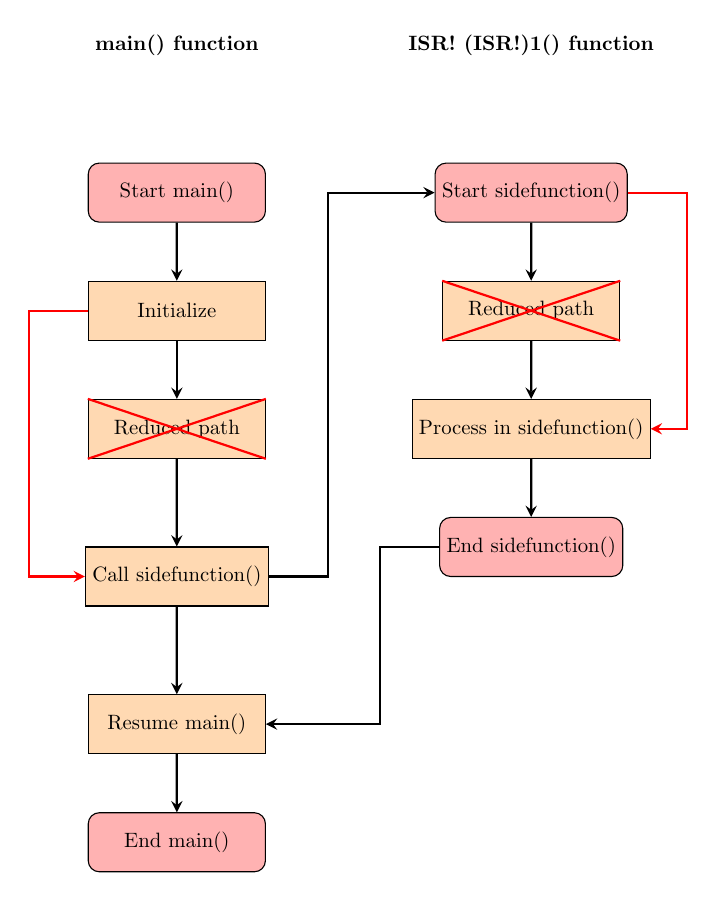
\begin{tikzpicture}[node distance=2cm, scale=0.75, transform shape]
				
				% Nodes for main function
				\node (start) [startstop] {Start main()};
				\node (init) [process, below of=start] {Initialize};
				\node (unimportant_main) [process, below of=init] {Reduced path};
				\node (callisr1) [process, below of=unimportant_main, yshift=-0.5cm] {Call sidefunction()};
				\node (resume) [process, below of=callisr1, yshift=-0.5cm] {Resume main()};
				\node (end) [startstop, below of=resume] {End main()};
				
				% Nodes for \ac{ISR}1 function
				\node (startisr1) [startstop, right of=callisr1, xshift=4cm, yshift=6.5cm] {Start sidefunction()};
				\node (unimportant_isr1) [process, below of=startisr1] {Reduced path};
				\node (processisr1) [process, below of=unimportant_isr1] {Process in sidefunction()};
				\node (endisr1) [startstop, below of=processisr1] {End sidefunction()};
				
				% Arrows for main function
				\draw [arrow] (start) -- (init);
				\draw [arrow] (init) -- (unimportant_main);
				\draw [arrow] (unimportant_main) -- (callisr1);
				\draw [arrow] (callisr1) -- (resume);
				\draw [arrow] (resume) -- (end);
				
				% Arrows for \ac{ISR}1 function
				\draw [arrow] (startisr1) -- (unimportant_isr1);
				\draw [arrow] (unimportant_isr1) -- (processisr1);
				\draw [arrow] (processisr1) -- (endisr1);
				
				% Interprocedural arrows
				\draw [arrow] (callisr1.east) -- ++(1,0) |- (startisr1);
				\draw [arrow] (endisr1.west) -- ++(-1,0) |- (resume);
				
				% Red arrows bypassing unimportant information
				\draw [redarrow] (init.west) -- ++(-1,0) |- (callisr1.west);
				\draw [redarrow] (startisr1.east) -- ++(1,0) |- (processisr1.east);
				
				% Red crosses over unimportant information
				\draw[red,thick] (unimportant_main.north west) -- (unimportant_main.south east);
				\draw[red,thick] (unimportant_main.north east) -- (unimportant_main.south west);
				\draw[red,thick] (unimportant_isr1.north west) -- (unimportant_isr1.south east);
				\draw[red,thick] (unimportant_isr1.north east) -- (unimportant_isr1.south west);
				
				% Labels
				\node [above of=start, yshift=0.5cm, text centered] {\textbf{main() function}};
				\node [above of=startisr1, yshift=0.5cm, xshift=0cm, text centered] {\textbf{\ac{ISR}1() function}};
				
			\end{tikzpicture}
			\caption{Example of a Reduced Inter-Procedural Control Flow Graph}
		\end{figure}
		
		Figure 2.3 shows an example of a simple reduction by eliminating nodes that do not carry any important information for the analysis the RICFG is used for. 
		
		\subsection{Depth-First Search}
		\ac{DFS} is an algorithm used to traverse a graph systematically. It begins at a source node and extends its exploration through the connected nodes as far as possible before it backtracks. In an algorithm this can be implemented using a recursive approach. The basic idea is to mark a node when its first discovered and then explore all the adjacent nodes that are not visited before. 
		\begin{figure}[H]
			\centering
			\begin{algorithm}[H]
				\SetAlgoLined
				\SetKwFunction{FMain}{dfs\_main}
				\SetKwFunction{DFS}{dfs}
				\SetKwProg{Fn}{Function}{:}{}
				
				\Fn{\DFS{node, visited}}{
					visited[node] = True\;
					\For{neighbor \textbf{in} graph[node]}{
						\If{not visited[neighbor]}{
							\DFS{neighbor, visited}\;
						}
					}
				}
			\end{algorithm}
			\caption{Example Implemenation of a Depth-First Search}
		\end{figure}
		In Figure 2.4 a simple example of a \ac{DFS} is shown. The \texttt{dfs} function gets called with the root node of a tree and performs the \ac{DFS} starting from the given node. It recursively calls itself with a new node called \texttt{neighbor} and repeats this until all the reachable nodes are marked as visited \cite{mehl2008}.
		
		
		\section{Data Races}
		
		A data race occurs when two or more functions or threads access a shared resource concurrently, without being ordered by a happens-before relationship, and one of those accesses is a write operation \cite{chen2011}. This can lead to unpredictable behavior and errors in the system, which makes the detection of data races a critical aspect of concurrent programs. Without proper synchronization, a system with multiple threads or functions that use shared data will lead to data races. The outcome of a program with data races is non-deterministic \cite{chen2011}. The order of execution of operations can vary, which may result in the generation of bugs that are not reproducible or difficult to reproduce. 
		
		\begin{figure}[H]
			\centering
			\begin{algorithm}[H]
				\caption{Data Race Example}
				\KwData{long shared1;}
				
				\BlankLine
				\SetKwFunction{FMain}{main}
				\SetKwProg{Fn}{Function}{:}{}
				\Fn{\FMain()}{
					\BlankLine
					\textbf{Variables}:\\
					unsigned char tmp\;
					\BlankLine
					\textbf{Code}:\\
					tmp $\leftarrow$ shared1\;
				}
				
				\BlankLine
				\SetKwFunction{FIsr}{isr1}
				\Fn{\FIsr()}{
					\BlankLine
					\textbf{Code}:\\
					idlerun()\;
					shared1 $\leftarrow$ 1\;
					idlerun()\;
				}
			\end{algorithm}
			\caption{Simple Example of a Data Race}
		\end{figure}
		
		In Figure 2.4, an example of a simple data race is shown. A global variable shared1 is initiated and accessed in two different functions, main() and isr1(). Since there are no synchronization tools used and the operation in isr1 is a write, there is a data race between line 5 and line 9.
		
		\subsection{Detection Techniques}
		
		Data race detection can be approached by two different analytical methods. Each of these methods provides benefits and challenges.
		
		\subsubsection{Static Data Race Detection \cite{wang2020}}
		\textbf{Advantages:}
		\begin{itemize}
			\item Comprehensiveness: Static analysis inspects the code without executing the program by analyzing every possible execution path and interaction that could lead to data races.
			\item Early Detection: Since static analysis does not require execution, it can analyze the code in the development phase, allowing the developer to find issues without deployment.
		\end{itemize}
		\textbf{Disadvantages:}
		\begin{itemize}
			\item False Positives/Negatives: Static analysis reports all data races that fall under certain conditions. Some of these data races could be very unlikely or even impossible at runtime. On the other hand, due to the approximations and assumptions necessary for tractability, it may miss some races.
			\item Complexity in Handling Dynamic Behavior: Dynamic behaviors such as pointers or recursion can be challenging to analyze for static approaches, leading to incomplete or inaccurate results.
		\end{itemize}
		
		\subsubsection{Dynamic Data Race Detection \cite{flanagan2009}}
		\textbf{Advantages:}
		\begin{itemize}
			\item Precision: Dynamic analysis tools monitor the actual execution of a program, identifying data races in real-time, which reduces the number of false positives.
			\item Context-Sensitive Detection: By analyzing the actual runtime behavior, dynamic analysis can understand the context of operations, leading to more accurate detection.
		\end{itemize}
		\textbf{Disadvantages:}
		\begin{itemize}
			\item Performance Overhead: The analysis at runtime can slow down the application significantly.
			\item Coverage: The effectiveness is heavily dependent on the execution path triggered during the tests. If certain parts of the program are not passed through in the execution run, they are not analyzed.
		\end{itemize}
		
		Both static and dynamic analyses are crucial for a complete analysis of code. They complement each other's limitations. A combination of both is the best approach to detecting data races most reliably. However, in this work, I am going to focus on the static analysis of data races.
		
		\subsection{Strategies for Preventing Data Races}
		
		Preventing data races requires careful design and implementation of concurrent programs. Effective strategies for general prevention of data races are synchronization mechanisms such as mutexes, semaphores, and condition variables, which control access to shared data. These mechanisms ensure that only one thread can access the shared resource at a time \cite{herlihy2008}. Since I am focusing on data races in interrupt-driven systems, the main tool to prevent data races is to disable \acp{ISR}, which access shared resources in critical areas.
		
		
		\begin{figure}[H]
			\centering
			\begin{algorithm}[H]
				\caption{Enable/Disable \ac{ISR} Call Example}
				\KwData{long shared1}
				
				\SetKwFunction{FMain}{main}
				\SetKwProg{Fn}{Function}{:}{}
				
				\Fn{\textbf{main()}}{
					\textbf{Variables}:\\
					unsigned char tmp\;
					\BlankLine
					\textbf{Code}:\\
					disable\_isr(1)\;
					tmp $\leftarrow$ shared1\;
					enable\_isr(1)\;
				}
				
				\Fn{\textbf{isr1()}}{
					\textbf{Code}:\\
					idlerun()\;
					shared1 $\leftarrow$ 1\;
					idlerun()\;
				}
				
				\Fn{\textbf{isr2()}}{
					\textbf{Code}:\\
					idlerun()\;
					int variable1 = 1\;
					idlerun()\;
				}
			\end{algorithm}
			\caption{Example of a Data Race with Enable/Disable \ac{ISR} Calls}
		\end{figure}
		
		Figure 2.5 is an example of a disable \ac{ISR} call that leads to the safe access of the shared data. The main function and isr1 both access the shared resource shared1. Since the read operation in line 6 of the main function is safely accessed by disabling isr1 in line 5 and enabling it in line 7, a possible data race is prevented.
		
		\section{Static Detection of Data Races in Interrupt-Driven Systems}
		
		The asynchronous nature and concurrent execution of \acp{ISR} and the main function introduce significant challenges for data consistency and detecting data races in interrupt-driven systems. Static data race analysis, especially those using \acp{RICFG}, is a promising approach to identifying data races without the need for extensive testing and runtime monitoring as in dynamic approaches \cite{wang2020}.
		
		The static approach involves the construction of an \ac{RICFG} for the program, which includes both the main code and \acp{ISR}, and capturing the control flow and potential interaction between them. Analyzing the \ac{RICFG} shows paths where shared resources are accessed concurrently without proper synchronization and indicates potential data races. Integrating the static analysis tool with the development process enables continuous detection of data races during software development, improving the reliability and correctness of interrupt-driven systems \cite{wang2020}.
		
		The methodology for static data race detection in interrupt-driven systems involves the following key steps. First, the \acp{RICFG} are constructed for the entire program, including the main code and the \acp{ISR}. This involves analyzing the control flow and identifying interactions between the main program and \acp{ISR}. Next, the \acp{RICFG} are analyzed to find potential data races, focusing on paths where concurrent access to shared data is done without proper synchronization. Finally, the developer can use the analysis results to address identified data races early in the development process \cite{wang2020}.
		
		
		\begin{figure}[H]
			\begin{algorithm}[H]
				\caption{Static Race Detection}
				\KwIn{RICFGs of P}
				\KwOut{potential racing pairs (PR)}
				
				\BlankLine
				\For{each $< G_i ; G_j >$ in RICFGs}{
					\For{each $sv_i \in G_i$}{
						\For{each $sv_j \in G_j$}{
							\If{$sv_i.V == sv_j.V$ and $(sv_i.A == W$ or $sv_j.A == W)$ and $G_i.pri < G_j.pri$ and $INTB.get(svi).contains(Gj)$}{
								$PR = PR \cup \{ <sv_i, sv_j> \}$\;
							}
						}
					}
				}
			\end{algorithm}
			\caption{Static Race Detection Approach by \cite{wang2020}}
		\end{figure}
		
		The approach by Wang et al. shows a computation of potential data races using \acp{RICFG}. By running a depth-first search on the \acp{RICFG}, it finds the interrupt status of every instruction. If there is a shared resource in both of the analyzed \acp{RICFG}, at least one of them is a write operation, and the two functions differ in their priority. While the interrupt in this pair is enabled, the two accesses are a potential data race \cite{wang2020}.
		
		In the following, I am going to introduce you to the implementation of my static analysis program based on the static race detection approach of Wang et al.
		
		
		
		\chapter{Implementation}
		In the following, I will provide an in-depth explanation of my implementation. For the generation of the input, I used \ac{GCC}. The command \texttt{gcc -fdump-tree-cfg} provides a cfg-file with all the important information for the intended data race analysis. I have split the explanation of the implementation into the initialization of the basic block class, the parsing of the input, the actual data race analysis, and the filtering of false positives found in data race analysis.
		
		
		\subsection*{Class BasicBlock}
		\begin{figure}[H]
			\centering
			\begin{algorithm}[H]
				\caption{BasicBlock Constructor}
				\DontPrintSemicolon
				\SetAlgoLined
				\KwData{function\_name, number, priority, shared\_resources, successors, enable\_disable\_calls, function\_calls}
				\KwResult{A BasicBlock object}
				\SetKwInOut{Input}{input}\SetKwInOut{Output}{output}
				\KwIn{function\_name, number, priority, shared\_resources (optional), successors (optional), enable\_disable\_calls (optional), function\_calls (optional)}
				\KwOut{A BasicBlock object}
				\BlankLine
				
				\SetKwFunction{FMain}{BasicBlock}
				\SetKwProg{Fn}{Function}{:}{}
				\Fn{\FMain{function\_name, number, priority, shared\_resources, successors, enable\_disable\_calls, function\_calls}}{
					self.function\_name $\gets$ function\_name\;
					self.number $\gets$ number\;
					self.priority $\gets$ priority\;
					self.shared\_resources $\gets$ shared\_resources \textbf{if} shared\_resources \textbf{else} empty list\;
					self.successors $\gets$ successors \textbf{if} successors \textbf{else} empty list\;
					self.enable\_disable\_calls $\gets$ enable\_disable\_calls \textbf{if} enable\_disable\_calls \textbf{else} empty list\;
					self.function\_calls $\gets$ function\_calls \textbf{if} function\_calls \textbf{else} empty list\;
				}
			\end{algorithm}
			
			\caption{Algorithm: Class BasicBlock}
		\end{figure}
		\vspace{1cm}
		
		The class \texttt{BasicBlock} displays all the information necessary for the data race analysis found in the input. This information includes the following attributes:
		\begin{itemize}
			\item \texttt{function\_name}: The function name to which the basic block belongs.
			\item \texttt{number}: The number of the basic block.
			\item \texttt{shared\_resources}: All accesses of shared resources within the \ac{BB}. The access type (read/write) and the line number of such calls are saved.
			\item \texttt{successors}: A list of all the successors of each basic block. Important for building all possible paths through the CFG.
			\item \texttt{enable\_disable\_calls}: All calls that disable or enable an \ac{ISR} within this basic block and also the corresponding line number of those calls to ensure the correct order.
			\item \texttt{function\_calls}: The functions that are called within a \ac{BB}.
		\end{itemize}
		Resulting in the following UML class diagramm:
		\begin{figure}[H]
			\centering
			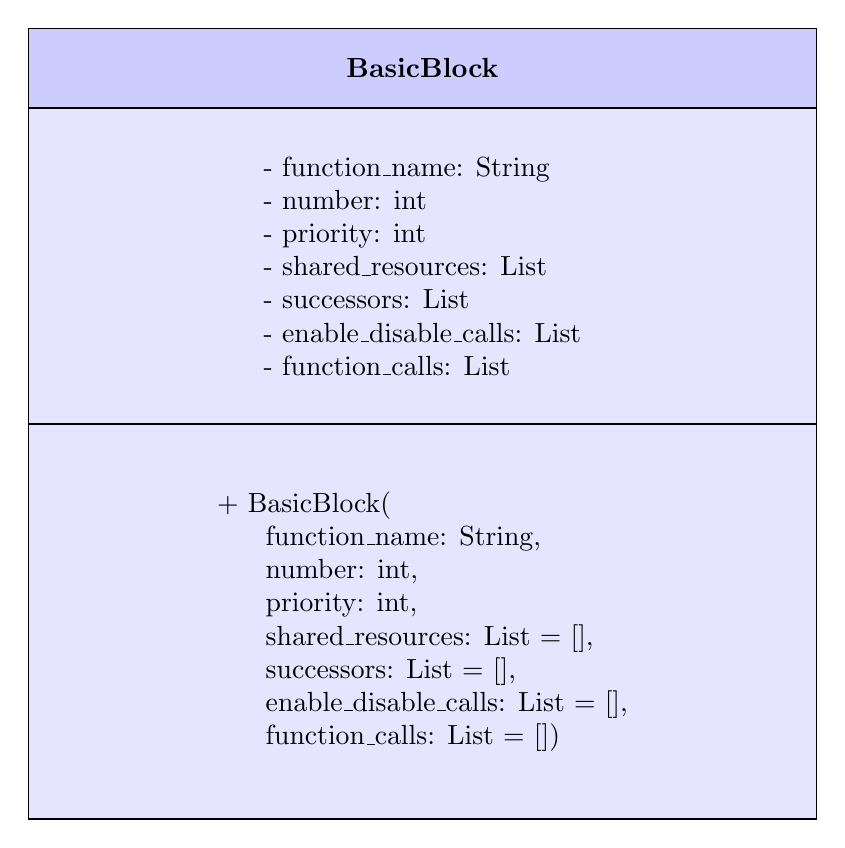
\begin{tikzpicture}
				% Define styles for the different elements of the class diagram
				\tikzstyle{class} = [rectangle, draw, minimum width=10cm, minimum height=1cm, font=\bfseries, fill=blue!20]
				\tikzstyle{attributes} = [rectangle, draw, minimum width=10cm, minimum height=4cm, anchor=north, align=left, fill=blue!10]
				\tikzstyle{methods} = [rectangle, draw, minimum width=10cm, minimum height=5cm, anchor=north, align=left, fill=blue!10]
				
				% Class name
				\node[class] (classname) at (0, 0) {BasicBlock};
				
				% Attributes
				\node[attributes, below=0cm of classname] (attributes) {
					- function\_name: String\\
					- number: int\\
					- priority: int\\
					- shared\_resources: List\\
					- successors: List\\
					- enable\_disable\_calls: List\\
					- function\_calls: List
				};
				
				% Methods
				\node[methods, below=0cm of attributes] (methods) {
					+ BasicBlock(\\
					\hspace*{5mm} function\_name: String,\\
					\hspace*{5mm} number: int,\\
					\hspace*{5mm} priority: int,\\
					\hspace*{5mm} shared\_resources: List = [],\\
					\hspace*{5mm} successors: List = [],\\
					\hspace*{5mm} enable\_disable\_calls: List = [],\\
					\hspace*{5mm} function\_calls: List = [])
				};
				
				% Draw the borders
				\draw (classname.north west) rectangle (methods.south east);
				\draw (attributes.north west) -- (attributes.north east);
				\draw (methods.north west) -- (methods.north east);
			\end{tikzpicture}
			\caption{UML: Class BasicBlock}
		\end{figure}
		
		
		\subsection*{Data Race Detection}
		The following functions are used to determine all possible data races, which are filtered later in the code. The intention is to find all possible data races to minimize the number of false negatives. Since false positives can be evaluated later by interpreting the output.
		
		
		\begin{figure}[H]
			\centering
			\begin{algorithm}[H]
				\caption{Initialization and ISR Enabling Map}
				\DontPrintSemicolon
				\SetAlgoLined
				\KwData{blocks}
				\KwResult{List of potential data races identified}
				\SetKwInOut{Input}{input}\SetKwInOut{Output}{output}
				\KwIn{Dictionary of BasicBlocks}
				\KwOut{List of potential data races}
				\BlankLine
				potential\_data\_races $\gets$ empty list\;
				resource\_accesses $\gets$ initialize as a default dictionary to list\;
				isr\_enabling\_map $\gets$ initialize as a default dictionary to set\;
				\BlankLine
				\ForEach{block in blocks}{
					\ForEach{call, line\_number in block.enable\_disable\_calls}{
						\If{call contains 'enable\_isr'}{
							isr\_idx\_match $\gets$ search for pattern '\(\d+\)' in call\;
							\If{isr\_idx\_match is found}{
								enabled\_isr\_idx $\gets$ integer value of the first group in isr\_idx\_match minus one\;
								enabler\_isr $\gets$ block.function\_name\;
								isr\_enabling\_map[enabler\_isr].add(enabled\_isr\_idx)\;
							}
						}
					}
				}
			\end{algorithm}
			\caption{Algorithm: Initialization and ISR Enabling Map}
		\end{figure}
		\vspace{1cm}
		
		
		The first part of the function \texttt{detect\_data\_races} takes a list of all basic block items as input. It also initializes the empty list of \texttt{potential\_data\_races}, a dictionary for \texttt{resource\_access}, and a dictionary for the \texttt{isr\_enabling\_map}. \texttt{Potential\_data\_races} and \texttt{resource\_access} are used later in the code. The main loop of the function iterates through every item in blocks and finds basic blocks with \texttt{enable\_disable\_calls}. If there is an enable call in a block item, the index of the enabled \ac{ISR} is read, and the basic block is added to the \texttt{isr\_enabling\_map} with the information on which \ac{ISR} it enables.
		
		\begin{figure}[H]
			\centering
			\begin{algorithm}[H]
				\caption{Process Block}
				\DontPrintSemicolon
				\SetAlgoLined
				\KwData{block, current\_isr\_status}
				\KwResult{Updated \ac{ISR} status and recorded resource accesses}
				\SetKwInOut{Input}{input}\SetKwInOut{Output}{output}
				\KwIn{A code block and the current \ac{ISR} status as a list}
				\KwOut{Updated current \ac{ISR} status and appended resource accesses to a global list}
				\BlankLine
				\ForEach{line, line\_number in block.code}{
					\If{line contains 'enable\_isr' or 'disable\_isr'}{
						isr\_idx\_match $\gets$ search for pattern '\(\d+\)' in line\;
						\If{isr\_idx\_match is found}{
							isr\_idx $\gets$ integer value of the first group in isr\_idx\_match minus one\;
							\eIf{"disable\_isr" is in line}{
								\If{0 $\leq$ isr\_idx $<$ length of current\_isr\_status}{
									current\_isr\_status[isr\_idx] $\gets$ 1\;  % Assuming 1 indicates disabled
								}
							}{
								\If{0 $\leq$ isr\_idx $<$ length of current\_isr\_status}{
									current\_isr\_status[isr\_idx] $\gets$ 0\;  % Assuming 0 indicates enabled
								}
							}
						}
					}
					\ForEach{resource\_name, access\_type, res\_line\_number in block.shared\_resources}{
						\If{res\_line\_number == line\_number}{
							resource\_accesses[resource\_name].append((block.function\_name, block.number, access\_type, line\_number, current\_isr\_status.copy()))\;
						}
					}
				}
			\end{algorithm}
			\caption{Algorithm: Process Block}
		\end{figure}
		\vspace{1cm}
		
		This part of the code runs through each line of a basic block to find the current \ac{ISR} status while resources are accessed. When a resource is found, all the information is added to the \texttt{resource\_accesses} dictionary, which includes the function name and the block number of the current basic block, as well as the access type, the line number, and the \ac{ISR} status of the access. All this information is used later for the detection of data races.
		
		\begin{figure}[H]
			\centering
			\begin{algorithm}[H]
				\caption{Depth-First Search (DFS) and Initialization}
				\DontPrintSemicolon
				\SetAlgoLined
				\KwData{blocks}
				\KwResult{Updated block ISR statuses and processed blocks}
				\SetKwInOut{Input}{input}\SetKwInOut{Output}{output}
				\KwIn{Dictionary of basic blocks}
				\KwOut{Updated block ISR statuses}
				\BlankLine
				
				\SetKwProg{Fn}{Function}{:}{}
				\Fn{dfs(block, visited\_blocks, current\_isr\_status, path)}{
					\If{(block.function\_name, block.number) \textbf{in} visited\_blocks}{
						block\_isr\_statuses[(block.function\_name, block.number)] $\gets$ merge\_isr\_statuses(block\_isr\_statuses[(block.function\_name, block.number)], current\_isr\_status)\;
						\Return\;
					}
					visited\_blocks.add((block.function\_name, block.number))\;
					path.append((block.function\_name, block.number))\;
					
					block\_isr\_statuses[(block.function\_name, block.number)] $\gets$ current\_isr\_status.copy()\;
					process\_block(block, current\_isr\_status)\;
					
					\If{not block.successors}{
						\Return\;
					}
					\Else{
						\For{successor \textbf{in} block.successors}{
							dfs(successor, set(visited\_blocks), current\_isr\_status.copy(), path.copy())\;
						}
					}
				}
				
				\BlankLine
				\tcp{Initialization and starting DFS from basic blocks with number 2}
				\For{(func\_name, bb\_num), block \textbf{in} blocks.items()}{
					\If{bb\_num == 2}{
						initial\_isr\_status $\gets$ track\_isr\_status(blocks).copy()\;
						process\_block(block, initial\_isr\_status)\;
						\For{successor \textbf{in} block.successors}{
							dfs(successor, set(), initial\_isr\_status.copy(), [(func\_name, bb\_num)])\;
						}
					}
				}
			\end{algorithm}
			\caption{Algorithm: \ac{DFS} and Initialization}
		\end{figure}
		\vspace{1cm}
		
		The \texttt{Depth-First Search (DFS)} function is recursively processing each block in a possible path of the \ac{RICFG}. The set \texttt{visited\_blocks} is used to avoid revisiting already visited blocks. If the block is already visited, the \ac{ISR} status is updated with the stored \ac{ISR} status for that block using the \texttt{merge\_isr\_statuses} function.
		
		\begin{figure}[H]
			\centering
			\begin{algorithm}[H]
				\caption{Merge ISR Statuses}
				\DontPrintSemicolon
				\SetAlgoLined
				\KwData{isr\_status1, isr\_status2}
				\KwResult{Merged ISR status list}
				\SetKwInOut{Input}{input}\SetKwInOut{Output}{output}
				\KwIn{Two lists of ISR statuses}
				\KwOut{List of merged ISR statuses}
				\BlankLine
				merged\_status $\gets$ empty list\;
				\For{isr1, isr2 \textbf{in} zip(isr\_status1, isr\_status2)}{
					merged\_status.append(min(isr1, isr2))\;
				}
				\Return{merged\_status}\;
			\end{algorithm}
			\caption{Algorithm: Merge \ac{ISR} Statuses}
		\end{figure}
		\vspace{1cm}
		
		This function takes the worst case of the most enabled \acp{ISR} and uses this for further analysis of the path.
		
		Unvisited blocks get added to the \texttt{visited\_blocks} set and to the path list. After that, the \ac{ISR} status gets updated to the current \ac{ISR} status, and the function \texttt{process\_block} is called to update the \ac{ISR} status and track the shared resource accesses.
		
		When the block is processed, the function checks for possible successors and recursively calls itself with the successor and the updated copy of \texttt{visited\_blocks}, \texttt{current\_isr\_status}, and the path.
		
		The first \ac{BB} in a function is always the \ac{BB} with number two in the generated cfg-files. To initialize the \ac{DFS}, the \ac{BB} number 2 is processed by the \texttt{process\_block} function, and after that, the \ac{DFS} function is called with the successor of the current block.
		
		
		\begin{figure}[H]
			\centering
			\begin{algorithm}[H]
				\caption{Check for Data Races}
				\DontPrintSemicolon
				\SetAlgoLined
				\KwData{resource\_accesses}
				\KwResult{List of potential data races}
				\SetKwInOut{Input}{input}\SetKwInOut{Output}{output}
				\KwIn{Dictionary of resource accesses}
				\KwOut{List of potential data races}
				\BlankLine
				\SetKwFunction{FMain}{check\_for\_data\_races}
				\SetKwProg{Fn}{Function}{:}{}
				\Fn{\FMain{}}{
					\For{resource, accesses \textbf{in} resource\_accesses.items()}{
						\For{i, (func1, bb\_num1, access\_type1, line\_number1, isr\_status1, priority1) \textbf{in} enumerate(accesses)}{
							\For{j, (func2, bb\_num2, access\_type2, line\_number2, isr\_status2, priority2) \textbf{in} enumerate(accesses)}{
								\If{i $\geq$ j}{
									Continue\;
								}
								\If{func1 $\neq$ func2 \textbf{and} (access\_type1 == "write" \textbf{or} access\_type2 == "write") \textbf{and} priority1 $\neq$ priority2}{
									potential\_data\_races.append((resource, (func1, bb\_num1, access\_type1, line\_number1, isr\_status1, priority1),
									(func2, bb\_num2, access\_type2, line\_number2, isr\_status2, priority2)))\;
								}
							}
						}
					}
				}
				\tcp{Call the function to check for data races}
				checkForDataRaces()\;
			\end{algorithm}
			\caption{Algorithm: Check for Data Races}
		\end{figure}
		\vspace{1cm}
		
		The function \texttt{check\_for\_data\_races} identifies potential data races by comparing the pairs of data accesses that were initiated earlier. It iterates through all possible tuples of accesses. If a tuple is not within the same function, one of the two accesses is a write operation, and the priorities of both accesses are different, the pair is added to the list of possible data races. All the items in the list fulfill the conditions of a possible data race, which do not include the \ac{ISR} status tracking. Since the \ac{ISR} status tracking is the more complex part of the analysis, this makes sure to find all possible data races before filtering to minimize the number of false negatives.
		
		
		
		\subsection*{Filter Possible Data Races}
		
		\begin{figure}[H]
			\centering
			\begin{algorithm}[H]
				\caption{Filter Data Races}
				\DontPrintSemicolon
				\SetAlgoLined
				\KwData{potential\_data\_races, isr\_enabling\_map}
				\KwResult{Filtered list of data races}
				\SetKwInOut{Input}{input}\SetKwInOut{Output}{output}
				\KwIn{List of potential data races, ISR enabling map}
				\KwOut{List of filtered data races}
				\BlankLine
				
				filtered\_data\_races $\gets$ empty list\;
				seen\_races $\gets$ empty set\;
				
				\For{resource, access1, access2 \textbf{in} potential\_data\_races}{
					func1, bb\_num1, access\_type1, line\_number1, isr\_status1, priority1 $\gets$ access1\;
					func2, bb\_num2, access\_type2, line\_number2, isr\_status2, priority2 $\gets$ access2\;
					
					relevant\_isr\_disabled1 $\gets$ is\_isr\_disabled(isr\_status1, func2) \textbf{and} not is\_isr\_enabled\_by\_another(isr\_status1, func2)\;
					relevant\_isr\_disabled2 $\gets$ is\_isr\_disabled(isr\_status2, func1) \textbf{and} not is\_isr\_enabled\_by\_another(isr\_status2, func1)\;
					
					race\_key $\gets$ frozenset(((func1, line\_number1), (func2, line\_number2)))\;
					
					\If{not (relevant\_isr\_disabled1 \textbf{or} relevant\_isr\_disabled2) \textbf{and} race\_key not \textbf{in} seen\_races}{
						filtered\_data\_races.append((resource, access1, access2))\;
						seen\_races.add(race\_key)\;
					}
				}
				
				\Return{filtered\_data\_races}\;
			\end{algorithm}
			\caption{Algorithm: Filter Data Races}
		\end{figure}
		\vspace{1cm}
		
		The \texttt{filter\_data\_races} function takes the list of possible data races given by the \texttt{check\_for\_data\_races} function and filters the racing pairs considering the \ac{ISR} statuses of the involved \acp{ISR}. It takes the two accesses of a potential race and extracts the information that is saved in those accesses. After that, it uses two helper functions to determine the \ac{ISR} statuses during the access.
		
		
		\begin{figure}[H]
			\centering
			\begin{algorithm}[H]
				\caption{Is ISR Disabled}
				\DontPrintSemicolon
				\SetAlgoLined
				\KwData{isr\_status, func\_name}
				\KwResult{Boolean indicating if the ISR is disabled}
				\SetKwInOut{Input}{input}\SetKwInOut{Output}{output}
				\KwIn{List of ISR statuses, function name as a string}
				\KwOut{Boolean}
				\BlankLine
				
				isr\_idx $\gets$ extract\_isr\_index(func\_name)\;
				\If{isr\_idx is not None \textbf{and} isr\_idx $<$ length of isr\_status}{
					\Return{isr\_status[isr\_idx] == 1}\;
				}
				\Return{False}\;
			\end{algorithm}
			\caption{Algorithm: Is \ac{ISR} Disabled}
		\end{figure}
		\vspace{1cm}
		
		The \texttt{is\_isr\_disabled} function checks if the bit corresponding to the \ac{ISR} in the \Ac{ISR} status array is set to one. If so, the function returns true to the \texttt{filter\_data\_races} function, and if not, it returns false. 
		
		\begin{figure}[H]
			\centering
			\begin{algorithm}[H]
				\caption{Is ISR Enabled by Another}
				\DontPrintSemicolon
				\SetAlgoLined
				\KwData{isr\_status, func\_name, isr\_enabling\_map}
				\KwResult{Boolean indicating if the ISR is enabled by another function}
				\SetKwInOut{Input}{input}\SetKwInOut{Output}{output}
				\KwIn{List of ISR statuses, function name as a string, ISR enabling map}
				\KwOut{Boolean}
				\BlankLine
				
				isr\_idx $\gets$ extract\_isr\_index(func\_name)\;
				\If{isr\_idx is not None}{
					\For{enabler\_isr, enabled\_isrs \textbf{in} isr\_enabling\_map.items()}{
						enabler\_idx $\gets$ extract\_isr\_index(enabler\_isr)\;
						\If{enabler\_idx is not None \textbf{and} not is\_isr\_disabled(isr\_status, enabler\_isr)}{
							\If{isr\_idx \textbf{in} enabled\_isrs}{
								\Return{True}\;
							}
						}
					}
				}
				\Return{False}\;
			\end{algorithm}
			\caption{Algorithm: Is \ac{ISR} Enabled by Another}
		\end{figure}
		\vspace{1cm}
		
		The \texttt{is\_isr\_enabled\_by\_another} function looks for possible activations of an \ac{ISR} by another \ac{ISR}. The \texttt{isr\_enabling\_map} was initiated and filled with information at the start of the \texttt{detect\_data\_races} function. This information is used in this function to determine if an \ac{ISR} is enabled by another \ac{ISR} that is enabled, to correctly handle racing pairs with these conditions.
		
		\newpage
		\subsection*{Parsing and Helper Functions}
		In this section the parsing of the input and the helper functions, which are called in the data race analysis, get explained.
		\begin{figure}[H]
			\scalebox{0.63}{
				\begin{algorithm}[H]
					\caption{Parse Basic Blocks}
					\DontPrintSemicolon
					\SetAlgoLined
					\KwData{file\_path, shared\_resource\_names}
					\KwResult{blocks, function\_blocks}
					\SetKwInOut{Input}{input}\SetKwInOut{Output}{output}
					\KwIn{Path to file, List of shared resource names}
					\KwOut{Dictionary of BasicBlocks, Dictionary of function blocks}
					\BlankLine
					Initialize variables\;
					lines $\gets$ read lines from file\;
					
					\For{line \textbf{in} lines}{
						line $\gets$ trim(line)\;
						
						\If{match function}{
							\If{bb\_num and current\_function}{
								Add BasicBlock to blocks and function\_blocks\;
							}
							current\_function $\gets$ extract function name\;
							bb\_num $\gets$ None\;
							Continue;
						}
						
						\If{match basic block}{
							\If{bb\_num and current\_function}{
								Add BasicBlock to blocks and function\_blocks\;
							}
							bb\_num $\gets$ extract basic block number\;
							Reset lists\;
						}
						
						\For{resource\_name \textbf{in} shared\_resource\_names}{
							\If{resource\_name \textbf{in} line}{
								\If{resource\_name is written}{
									Add write to shared\_resources\;
								}
								\Else{
									Add read to shared\_resources\;
								}
							}
						}
						
						\If{line contains enable\_isr or disable\_isr}{
							Add to enable\_disable\_calls\;
						}
						
						\If{match function call}{
							Add function call to function\_calls\;
						}
					}
					
					\If{bb\_num and current\_function}{
						Add BasicBlock to blocks and function\_blocks\;
					}
					
					\For{line \textbf{in} lines}{
						line $\gets$ trim(line)\;
						
						\If{match function}{
							current\_function $\gets$ extract function name\;
							bb\_num $\gets$ None\;
							Continue;
						}
						
						\If{line contains successors}{
							Extract successors and update BasicBlock successors\;
						}
					}
					
					\Return{blocks, function\_blocks}\;
				\end{algorithm}
				
			}
			\caption{Algorithm: Parse Basic Blocks}
		\end{figure}
		\vspace{1cm}
		The \texttt{parse\_basic\_block} function iterates two times through the code to extract all the important information of the code and save it in the \ac{BB} items. In the first iteration of the code lines, the \acp{BB} get initiated with the \ac{BB} number and the function it relates to. Additionaly the information of shared resources, enable/disable calls of \acp{ISR} and function calls within the \ac{BB} are added.
		In the second iteration the successors of the \ac{BB} get added. A second iteration is used to ensure all the \acp{BB} items are initialized first to ensure a correct handling of the successors.
		
		\begin{figure}[H]
			\centering
			\scalebox{1}{ % Adjust the value to your desired scale
				\begin{algorithm}[H]
					\caption{Determine Priority}
					\DontPrintSemicolon
					\SetAlgoLined
					\KwData{function\_name}
					\KwResult{Priority of the function}
					\SetKwInOut{Input}{input}\SetKwInOut{Output}{output}
					\KwIn{Function name as a string}
					\KwOut{Priority as an integer}
					\BlankLine
					match $\gets$ search for \textit{`isr\_?(\d+)' in function\_name}\;
					\If{match is found}{
						\Return{integer value of matched group} \tcp*[f]{Higher priority for lower ISR number}
					}
					\Else{
						\Return{infinity} \tcp*[f]{Lower priority for non-ISR functions}
					}
				\end{algorithm}
				
			}
			\caption{Algorithm: Determine Priority}
		\end{figure} 
		
		The \texttt{determine\_priority} function is used to determine the priority of the function which is involved in a possible data race. Since one condition for a data race is two different priorities of the function this is an important check. The priority gets determined in the first place by differentiate between \ac{ISR} functions and normal functions because \acp{ISR} always have a higher priority than non-\ac{ISR} functions. Non-\Ac{ISR} functions have the priority infinity and \acp{ISR} get ordered by the number of it, while lower number \acp{ISR} have a higher priority than higher number ones.
		
		\begin{figure}[H]
			\centering
			\scalebox{1}{ % Adjust the value to your desired scale
				\begin{algorithm}[H]
					\caption{Track ISR Status}
					\DontPrintSemicolon
					\SetAlgoLined
					\KwData{blocks}
					\KwResult{List indicating ISR status initialized to zero}
					\SetKwInOut{Input}{input}\SetKwInOut{Output}{output}
					\KwIn{Dictionary of BasicBlocks}
					\KwOut{List of zeros representing the status of each ISR}
					\BlankLine
					isr\_count $\gets$ count unique ISR function names in blocks\;
					\Return{list of zeros of length isr\_count}
				\end{algorithm}	
			}
			\caption{Algorithm: Track ISR Status}
		\end{figure} 
		
		\begin{figure}[H]
			\centering
			\scalebox{1}{ % Adjust the value to your desired scale
				\begin{algorithm}[H]
					\caption{Extract ISR Index}
					\DontPrintSemicolon
					\SetAlgoLined
					\KwData{function\_name}
					\KwResult{Index of the ISR}
					\SetKwInOut{Input}{input}\SetKwInOut{Output}{output}
					\KwIn{Function name as a string}
					\KwOut{ISR index as an integer}
					\BlankLine
					match $\gets$ search for ISR pattern in function\_name\;
					\If{match}{
						\Return{integer value of matched group minus one}
					}
					\Return{None}
				\end{algorithm}
				
			}
			\caption{Algorithm: Track ISR Status}
		\end{figure} 
		\begin{figure}[H]
			\centering
			\scalebox{1}{ % Adjust the value to your desired scale
				\begin{algorithm}[H]
					\caption{Propagate Function Calls}
					\DontPrintSemicolon
					\SetAlgoLined
					\KwData{blocks, function\_blocks}
					\KwResult{Updated blocks with propagated function call information}
					\SetKwInOut{Input}{input}\SetKwInOut{Output}{output}
					\KwIn{Dictionary of BasicBlocks, Dictionary of function blocks}
					\KwOut{Updated BasicBlocks with propagated resources and ISR calls}
					\BlankLine
					\For{each function \textbf{in} function\_blocks}{
						\For{each block \textbf{in} function's block list}{
							\For{each called\_func, line\_number \textbf{in} block's function calls}{
								\If{called\_func \textbf{in} function\_blocks}{
									\For{each called\_block \textbf{in} function\_blocks[called\_func]}{
										block.shared\_resources.extend(called\_block.shared\_resources)\;
										block.enable\_disable\_calls.extend(called\_block.enable\_disable\_calls)\;
									}
								}
							}
						}
					}
				\end{algorithm}
			}
			\caption{Algorithm: Propagate Function Calls}
		\end{figure} 
		The \texttt{propagate\_function\_calls} function is handling the case of a function that calls another function. It checks for \acp{BB} items with a function call in it and adds the critical parts of the called function to the current \ac{BB} to simulate a path through the called function and consider the shared resources and enable/disable calls of that function.
		
		\chapter{Evaluation}
		
		Done:\\
		-Data Race Detection with all necessary criterias for a data race\\
		-Informations of the cfg brought down to the minimum needed to analyze for data races\\
		-Inter-Procedural checks of function calls\\
		-Recursive traversion of the CFG using DFS\\
		-Implementation of an ISR Status Array that updates thorugh the traversal\\
		-Considering ISR enabling ISRs\\
		
		
		Not Done/ Future work:\\
		-Pointer analysis\\
		-Unnecessary nodes in CFG are empty but not deleted\\
		-ISR enabling ISR with a depth of more than one are not considered (1 activates 2 activates 3 and 3 has data race)\\
		\chapter{Conclusion}
		
		\appendix
	}
	\backmatter{}
	\begin{thebibliography}{9}
		\bibitem{wang2020}
		Wang, Y., Gao, F., Wang, L., Yu, T., Zhao, J., \& Li, X. (2020). Automatic Detection, Validation, and Repair of Race Conditions in Interrupt-Driven Embedded Software. IEEE Transactions on Software Engineering.
		
		\bibitem{engler2003}
		Engler, D., \& Ashcraft, K. (2003). RacerX: Effective, Static Detection of Race Conditions and Deadlocks. ACM SIGOPS Operating Systems Review.
		
		\bibitem{chopra2019}
		Nikita Chopra, Rekha Pai, and Deepak D’Souza (2019). Data Races and Static Analysis for Interrupt-Driven Kernels
		
		\bibitem{flanagan2009}
		Flanagan, C., \& Freund, S. N. (2009). FastTrack: Efficient and Precise Dynamic Race Detection. ACM SIGPLAN Notices.
		
		\bibitem{chen2011}
		R. Chen, Xiangying Guo, Y. Duan, B. Gu, Mengfei Yang (2011). Static Data Race Detection for Interrupt-Driven Embedded Software.
		
		\bibitem{muchnick1997}
		Muchnick, S. S. (1997). Advanced Compiler Design and Implementation. Morgan Kaufmann.
		
		\bibitem{adve1996}
		Adve, S. V., \& Gharachorloo, K. (1996). Shared Memory Consistency Models: A Tutorial. IEEE Computer.
		
		\bibitem{herlihy2008}
		Herlihy, M., \& Shavit, N. (2008). The Art of Multiprocessor Programming. Morgan Kaufmann.
		
		\bibitem{mehl2008}
		K. Mehlhorn, P. Sanders (2008). Algorithms and Data Structures The Basic Toolbox.
	\end{thebibliography}
	\chapter{Attachments}
	\begin{lstlisting}[language=Python, mathescape, escapeinside={(*}{*)}]
		class BasicBlock:
		def __init__(function_name, number, shared_resources=[], successors=[], enable_disable_calls=[], code=[]):
		self.function_name = function_name
		self.number = number
		self.shared_resources = shared_resources
		self.successors = successors
		self.enable_disable_calls = enable_disable_calls
		self.code = code
		
		def __repr__():
		return ("BasicBlock(function_name={}, number={}, shared_resources={}, "
		"successors={}, enable_disable_calls={}, code={})".format(
		self.function_name, self.number, self.shared_resources, 
		[succ.number for succ in self.successors], self.enable_disable_calls, 
		' '.join(self.code)))
		
		def parse_basic_blocks(file_path, shared_resource_names):
		blocks = {}
		current_function = None
		
		with open(file_path, 'r') as file:
		lines = file.readlines()
		
		bb_num = None
		shared_resources = []
		enable_disable_calls = []
		code_lines = []
		line_number = 0  
		
		for line in lines:
		line = line.strip()
		line_number += 1
		
		func_match = re.match(r';; Function (.+?) \(', line)
		if func_match:
		if bb_num is not None and current_function is not None:
		blocks[(current_function, bb_num)] = BasicBlock(
		current_function, bb_num, shared_resources, [], enable_disable_calls, code_lines)
		current_function = func_match.group(1)
		bb_num = None
		continue
		
		bb_match = re.match(r'<bb (\d+)>:', line)
		if bb_match:
		if bb_num is not None and current_function is not None:
		blocks[(current_function, bb_num)] = BasicBlock(
		current_function, bb_num, shared_resources, [], enable_disable_calls, code_lines)
		bb_num = int(bb_match.group(1))
		shared_resources = []
		enable_disable_calls = []
		code_lines = []
		
		for resource_name in shared_resource_names:
		if re.search(fr'\b{resource_name}\b', line):
		if re.search(fr'\b{resource_name}\b\s*=', line):
		shared_resources.append((resource_name, 'write', line_number))
		else:
		shared_resources.append((resource_name, 'read', line_number))
		
		if 'enable_isr' in line or 'disable_isr' in line:
		enable_disable_calls.append((line.strip(), line_number))
		
		code_lines.append((line, line_number))
		
		if bb_num is not None and current_function is not None:
		blocks[(current_function, bb_num)] = BasicBlock(
		current_function, bb_num, shared_resources, [], enable_disable_calls, code_lines)
		
		current_function = None
		bb_num = None
		for line in lines:
		line = line.strip()
		
		func_match = re.match(r';; Function (.+?) \(', line)
		if func_match:
		current_function = func_match.group(1)
		bb_num = None
		continue
		
		if 'succs' in line:
		succ_match = re.match(r';; (\d+) succs \{(.+?)\}', line)
		if succ_match:
		bb_num = int(succ_match.group(1))
		succ_list = [int(succ.strip()) for succ in succ_match.group(2).split()]
		if (current_function, bb_num) in blocks:
		blocks[(current_function, bb_num)].successors = [
		blocks[(current_function, succ)] for succ in succ_list if (current_function, succ) in blocks]
		
		return blocks
		
		def track_isr_status(blocks):
		isr_count = len(set(block.function_name for block in blocks.values() if re.search(r'isr[_]?\d+', block.function_name)))
		return [0] * isr_count  
		
		def extract_isr_index(function_name):
		match = re.search(r'isr[_]?(\d+)', function_name)
		if match:
		return int(match.group(1)) - 1
		return None
		
		def detect_data_races(blocks):
		potential_data_races = []
		resource_accesses = defaultdict(list)
		isr_enabling_map = defaultdict(set)
		
		for block in blocks.values():
		for call, line_number in block.enable_disable_calls:
		if 'enable_isr' in call:
		isr_idx_match = re.search(r'\((\d+)\)', call)
		if isr_idx_match:
		enabled_isr_idx = int(isr_idx_match.group(1)) - 1
		enabler_isr = block.function_name
		isr_enabling_map[enabler_isr].add(enabled_isr_idx)
		
		def process_block(block, current_isr_status):
		for line, line_number in block.code:
		if 'enable_isr' in line or 'disable_isr' in line:
		isr_idx_match = re.search(r'\((\d+)\)', line)
		if isr_idx_match:
		isr_idx = int(isr_idx_match.group(1)) - 1  
		if "disable_isr" in line:
		if 0 <= isr_idx < len(current_isr_status):
		current_isr_status[isr_idx] = 1
		elif "enable_isr" in line:
		if 0 <= isr_idx < len(current_isr_status):
		current_isr_status[isr_idx] = 0
		
		
		for resource_name, access_type, res_line_number in block.shared_resources:
		if res_line_number == line_number:
		resource_accesses[resource_name].append((block.function_name, block.number, access_type, line_number, current_isr_status.copy()))
		
		def dfs(block, visited_blocks, current_isr_status, path):
		if (block.function_name, block.number) in visited_blocks:
		return
		visited_blocks.add((block.function_name, block.number))
		path.append((block.function_name, block.number))
		
		process_block(block, current_isr_status)
		
		if not block.successors:
		pass
		else:
		for successor in block.successors:
		dfs(successor, set(visited_blocks), current_isr_status.copy(), path.copy())
		
		
		for (func_name, bb_num), block in blocks.items():
		if bb_num == 2:  
		initial_isr_status = track_isr_status(blocks).copy()
		process_block(block, initial_isr_status)
		for successor in block.successors:
		dfs(successor, set(), initial_isr_status.copy(), [(func_name, bb_num)])
		
		
		def check_for_data_races():
		for resource, accesses in resource_accesses.items():
		for i, (func1, bb_num1, access_type1, line_number1, isr_status1) in enumerate(accesses):
		for j, (func2, bb_num2, access_type2, line_number2, isr_status2) in enumerate(accesses):
		if i >= j:
		continue  
		if func1 != func2 and (access_type1 == "write" or access_type2 == "write"):
		potential_data_races.append((resource, (func1, bb_num1, access_type1, line_number1, isr_status1),
		(func2, bb_num2, access_type2, line_number2, isr_status2)))
		
		check_for_data_races()
		
		
		def filter_data_races(potential_data_races):
		filtered_data_races = []
		for resource, access1, access2 in potential_data_races:
		func1, bb_num1, access_type1, line_number1, isr_status1 = access1
		func2, bb_num2, access_type2, line_number2, isr_status2 = access2
		
		def is_isr_disabled(isr_status, func_name):
		isr_idx = extract_isr_index(func_name)
		if isr_idx is not None and isr_idx < len(isr_status):
		return isr_status[isr_idx] == 1
		return False
		
		def is_isr_enabled_by_another(isr_status, func_name):
		isr_idx = extract_isr_index(func_name)
		if isr_idx is not None:
		for enabler_isr, enabled_isrs in isr_enabling_map.items():
		enabler_idx = extract_isr_index(enabler_isr)
		if enabler_idx is not None and not is_isr_disabled(isr_status, enabler_isr):
		if isr_idx in enabled_isrs:
		return True
		return False
		
		relevant_isr_disabled1 = is_isr_disabled(isr_status1, func2) and not is_isr_enabled_by_another(isr_status1, func2)
		relevant_isr_disabled2 = is_isr_disabled(isr_status2, func1) and not is_isr_enabled_by_another(isr_status2, func1)
		
		if not (relevant_isr_disabled1 or relevant_isr_disabled2):
		filtered_data_races.append((resource, access1, access2))
		
		return filtered_data_races
		
		filtered_data_races = filter_data_races(potential_data_races)
		
		return filtered_data_races
		
		
		shared_resource_input = input("Enter the names of shared resources, separated by commas: ")
		shared_resource_names = [name.strip() for name in shared_resource_input.split(',')]
		
		file_path = input("Enter the file path: ").strip()
		blocks = parse_basic_blocks(file_path, shared_resource_names)
		
		data_races = detect_data_races(blocks)
		
		print("Detected Data Races:")
		for resource, access1, access2 in data_races:
		print(f"Resource: {resource}")
		print(f"  Access 1: Function {access1[0]} (BB {access1[1]}), {access1[2]}, Line {access1[3]}, ISR Status: {access1[4]}")
		print(f"  Access 2: Function {access2[0]} (BB {access2[1]}), {access2[2]}, Line {access2[3]}, ISR Status: {access2[4]}")
		print()
	\end{lstlisting}
\end{document}